\chapter{A Quantitative Evaluation of Energy Storage}
\label{chap:battery}

From the previous chapter, I have identified the value of properly sizing energy capacity in an energy harvesting design to increase energy capture and system reliability. 
Many modern energy harvesting sensor designs have utilized capacitors in their designs, which severely limit energy capacity.
Many modern platforms are attempting to push the energy bounds of sensing, computation and networking, and have begun incorporating supercapacitors to provide the necessary energy to make certain applications feasible~\cite{nardello2019camaroptera}.
These decisions are made despite the obvious option for energy capacity: batteries.
%Due to an increased need for energy storage to enable more advanced sensing and processing, the majority of modern batteryless research energy harvesting platforms utilize supercapacitors instead of tantalum or ceramic capacitors due to their superior energy density.
These designers have eschewed batteries as an option, despite their vastly superior energy density, dismissing them qualitatively as 
bulky~\cite{hesterNew17, hesterTragedy15, hesterFlicker17, hesterTimely17, yervaGrafting12},
inefficient~\cite{hesterNew17, hesterTragedy15, hesterFlicker17, hesterTimely17},
expensive~\cite{hesterNew17, hesterTragedy15, hesterFlicker17, hesterTimely17},
short-lived~\cite{hesterNew17, hesterTragedy15, hesterFlicker17, hesterTimely17, colinReconfigurable18, luciaIntermittent17, yervaGrafting12}.
%high-maintenance~\cite{hesterNew17, hesterTragedy15, hesterFlicker17, hesterTimely17, colinReconfigurable18, luciaIntermittent17},
temperature-sensitive~\cite{hesterNew17, hesterTragedy15, hesterFlicker17, hesterTimely17, colinReconfigurable18, luciaIntermittent17},
%difficult to monitor~\cite{hesterNew17, hesterTragedy15, hesterFlicker17, hesterTimely17, colinReconfigurable18, luciaIntermittent17},
%fragile~\cite{hesterNew17, hesterTragedy15, hesterFlicker17, hesterTimely17},
and dangerous~\cite{hesterNew17, hesterTragedy15, hesterFlicker17, hesterTimely17}. 
%These qualitative claims against batteries were valid when considering some of the first available rechargeable batteries. 
%Nickel Cadmium (NiCad) cells provide poor energy density, and a memory effect that prematurely reduces energy capacity if the cell is not discharged fully before recharging. Nickel Metal Hydride (NiMH) cells offer a higher capacity than NiCad without a memory effect, but have short cycle lifetimes, are heavy, and have higher self-discharge. Lithium-ion (Li-ion) cells offer the highest energy density of any battery chemistry, but continue to be limited by cycle lifetimes, as well as thermal runaway if mishandled.

In this chapter, I reexamine each of these arguments with respect to modern capacitor, supercapacitor, and battery technology. 
While the batteries of one or two decades ago were certainly guilty of the myriad of the complaints against them, new 
battery anode materials
, including lithium titanate oxide (LTO), 
lithium iron phosphate (LiFePO\textsubscript{4}), and improved lithium-ion manufacturing processes have produced extremely appealing options for energy storage when compared to capacitors and supercapacitors. 
New battery technology paired with newly available low power energy harvesting and battery management ICs~\cite{bq25505} enables the design of high-capacity energy harvesting systems.
Despite improvements, batteries still underperform in some metrics compared to supercapacitors, but these deficiencies are likely inconsequential for the majority of wireless sensor applications, and the substantial increase in energy capacity outweighs any detracting tradeoffs.\\

\placefigure{tab:battery:cost}

\section{Energy Storage Technology}
\label{sec:battery-new}

I summarize the notable characteristics of various examples of capacitors, supercapacitors, and batteries in \cref{tab:battery:cost}. The representative capacitors and supercapacitors in this table were chosen based on their inclusion in existing batteryless platforms, including the Solar Monjolo~\cite{campbellEnergy14}, Flicker~\cite{hesterFlicker17}, Capybara~\cite{colinReconfigurable18}, and Camaroptera~\cite{nardello2019camaroptera}.
The batteries represent some of the smallest lithium-based cells that are commercially available. 

\subsection{Ceramic and Tantalum Capacitors}
\subsection{Supercapacitors}
\subsection{LTO}
\subsection{LiFePO}
\subsection{Thin-film}
\subsection{Improved Li-ion}

\section{Volume and Density}
Arguments that deride batteries as bulky are likely directly comparing the size of a small battery to that of single tantalum or ceramic capacitor, without considering energy and power density. New miniature batteries are comparable in volume to many supercapacitors, and even a banked combination of ceramic and tantalum capacitors, while offering substantially more energy density and providing an acceptable power density. In this section, I explore the "bulkiness" of capacitors, supercapacitors, and batteries in the context of energy and power density. Here, I am considering volumetric density (\si[per-mode=symbol]{\Wh\per\liter}  and  \si[per-mode=symbol]{\watt\per\liter}) instead of specific energy and power (\si[per-mode=symbol]{\Wh\per\kilo\gram} and  \si[per-mode=symbol]{\watt\per\kilo\gram}, respectively) to better compare the volume of these energy storage options.

\subsection{Energy Density}
Energy density should be the primary consideration for energy harvesting power supply design to maximize energy capacity while simultaneously minimizing volume. 
The energy stored in a capacitor is calculated in one of two ways:

$$E_{eff_{cap}} = \frac{1}{2} C (V^2 - V_{min}^2)$$
$$E_{total_{cap}} = \frac{1}{2} C V^2$$

Where $E_{eff}$ and $E_{total}$ is the effective and total energy stored in a capacitor, respectively. These amounts are defined by the capacitor's capacitance $C$, and the applied voltage $V$, and the minimum voltage $V_{min}$. Usually $V_{min}$ represents the minimum to do something useful. Often this is the minimum open circuit voltage to cold start a boost regulator, between 400\si{\milli\volt} to 600\si{\milli\volt}~\cite{adp5091,bq25505,max17222}. 
For simplicity sake, I use $E_{total}$ to determine energy capacity and density. For most capacitors, the unusable energy represented by $E_{eff_{cap}}$ is negligible compared to the total energy. Likewise, energy stored in a battery is calculated as follows:

$$E_{bat} = Q V_{nom}$$

Where $Q$ is the charge capacity (often denoted in terms of \si{\Ah}) and $V_{nom}$ is the battery's nominal voltage. Nominal voltage represents an average of the battery's voltage curve over the course of a charge/discharge cycle. The nominal voltage and capacity of a battery are provided by the manufacturer and are almost always included in a datasheet.

A selection of capacitor, supercapacitor, and battery energy capacities and densities are summarized in \cref{tab:battery:cost}. Among this selection, small batteries are 50-1000x more energy dense than supercapacitors and three to five orders of magnitude more dense than ceramic and tantalum capacitors. Li-ion and LiPo chemistries are the most energy dense among batteries.

Several of these capacitors, supercapacitors and batteries are shown visually in \cref{fig:battery:sizes}.
The capacitor and supercapacitor configurations are based on examples from batteryless platform designs described in the literature~\cite{hesterFlicker17, campbellEnergy14,colinReconfigurable18}.
The batteries shown in \cref{fig:battery:sizes} are
as small as 88\si{\milli\meter\cubed}, and resemble small through-hole
capacitors and coin cells. Battery \textbf{(b)} is smaller in volume than many of the capacitor
configurations presented in the literature, only outdone by systems like Flicker \textbf{(a)} which utilize only a few ceramic capacitors~\cite{hesterFlicker17}.
This small LTO battery offers 3.7x 
more energy storage and 50x more energy density than the largest supercapacitor presented (\textbf{h}). When considering the size of other components in the system, most notably the harvester (solar panel, thermocouple, or piezoelectric device), the combination of ICs, and large sensors like a PIR motion sensor, the size of small rechargeable batteries is inconsequential. 
Even the smallest energy harvesting sensor system to our knowledge, the size of the entire Michigan Micro Mote~\cite{lee13modular} system is about the size of a single ceramic capacitor and utilizes a thin-film battery for energy storage. When considering energy density, capacitors and supercapacitors are significantly more bulky than batteries.

\placefigure{fig:battery:sizes}

\subsection{Power Density}
In addition to energy density, power density is also an important metric to consider for a design. 
Common wireless sensor workloads are characterized by very low sleep currents punctuated by infrequent pulses of high current, usually a radio transmission. Energy storage must provide sufficient power to drive these short pulses. The maximum delivered power is largely dependent on equivalent series resistance (ESR), represented by an internal series resistance to the capacitor or battery cell. 
Internal resistance for both supercapacitors and batteries is temperature and age dependent. Both storage elements experience increased ESR at temperature extremes, and experience increased ESR as they age.
The internal resistance of capacitors and supercapacitors is also frequency dependent, and usually reported for 1\si{\kilo\hertz}. This value is generally related inversely with frequency for frequencies below the capacitor's self-resonance~\cite{murataESRArticle}. For the relatively low frequency of charge/discharge cycles characteristic of energy harvesting devices, actual ESR is likely higher than reported.

Internal capacitor, supercapacitor, and battery resistance incurs a voltage drop over this resistance which is especially noticeable and detrimental during high power loads.
Ceramic and tantalum capacitors have negligible ESR and incomparably high power density, so I focus on comparing the power density of supercapacitors and batteries.
There are two different metrics for quantifying power output of supercapacitors and batteries. The first is effective power $P_{eff}$, and represents the maximum sustainable and continuous power that can be provided. The second is peak power $P_{max}$ and represents the maximum possible current that can be provided in short pulses. These metrics are defined differently for supercapacitors and batteries. For a supercapacitor, power output is defined as follows~\cite{IEC62391}:

$$P_{eff_{sc}} = \frac{1}{8} \frac{V^2}{R_i}$$
$$P_{max_{sc}} = \frac{1}{4} \frac{V^2}{R_i}$$

Where $V$ is the voltage applied to the capacitor, and $R_i$ is the internal resistance, or ESR. For batteries, these metrics are defined as follows:

$$P_{eff_{bat}} = I_{cont} V_{nom}$$
$$P_{max_{bat}} = I_{max} V_{nom}$$

Where $I_{cont}$ and $I_{max}$ are the battery's rated continuous and peak pulsed current respectively. These metrics are provided by the battery manufacturer and often included in the battery datasheet. The continuous and peak currents are often defined in terms of the C-rate, or a proportion of the rated capacity (in units of \si{\Ah}). For example, the 1C rate of a 100\si{\milli\Ah} battery is 100\si{\milli\ampere}, and the 2C rate is 200\si{\milli\ampere}. For sake of comparison, I use $P_{eff}$ in \cref{tab:battery:cost} for batteries and supercapacitors, as it is a more conservative measure of the energy storage power capability. 

Among the supercapacitors and batteries featured in \cref{tab:battery:cost}, supercapacitors provide 10-400x more power density. However, one supercapacitor outlier provides the least power density of all options. Despite their superior power density, I argue that most applications do not require the higher power density afforded by supercapacitors. It is hard to imagine a \textit{low power} energy harvesting application that must source more than a few to a few hundred milliamperes at 3\si{\volt} infrequently, nevermind continuously.
Conventional Li-ion and LiPo cells can generally source 1C continuously. The smallest Li-ion cell can provide 11\si{\milli\ampere} continuously, and the largest can provide 80\si{\milli\ampere}. The LiPo cell presented can supply 40\si{\milli\ampere} continuously. 
Small LTO and LiFePO\textsubscript{4} cells are capable of very high C-rates, often between 20-40C for LTOs, and 10-20C for LiFePO\textsubscript{4}~\cite{lifepo4Datasheet,LTODatasheet,LTODatasheet2}.
The smaller LTO battery listed in \cref{tab:battery:cost} is able to source 18\si{\milli\ampere}, while the larger LTO and LiFePO\textsubscript{4} cells can source 400-700\si{\milli\ampere} continuously. 
This power capability is more than sufficient for the majority of applications, either indoors with PANs, or outdoors, with cellular or LPWANs~\cite{nrf52840,ghena2019challenge}.

\placefigure{fig:battery:ragone}

\section{Efficiency}
\label{sec:supercapvbattery}
At a high level, the efficiency of an energy storage element can be defined as the actual proportion of stored energy that is used to perform a desired task or application. Batteries have been derided as "inefficient" by platform designers in the literature, however
both supercapacitor and battery technology exhibit the same two phenomena that causes inefficiency, and generally to the same extent. The first phenomena is power dissipation over the ESR of the device, which was mentioned in the previous section. The second is self-discharge or leakage, which can be represented by an internal parallel resistance to the capacitor or battery.
This section seeks to quantitatively compare these two sources of inefficiency for supercapacitors and batteries.

\subsection{Internal Resistance}
The power dissipated over the internal resistance, or ESR, can be calculated as follows:

$$P_{i} = R_{i} I^2$$

Due to the squared relationship of power to current, high current events, such as a radio transmission, are the primary cause of ESR power losses. The total power required to drive a load, including losses over internal resitance, can be described as:

$$P_{total} = P_{l} + P_{i}$$
$$P_{total} =  I V + R_{i} I^2$$

Where $I$ and $V$ are the current and voltage required to drive an intended load.
With a subset of the
capacitors and batteries mentioned in \cref{tab:battery:cost}, an 8\si{\milli\ampere} BLE
transmission from a steady 3\,V would incur less
than 0.03\% in resistive loss from a tantalum capacitor, a 2.1\% loss from the 1.8\si{\milli\Ah} LTO battery, and 6.3\% loss from the 7.5\si{\milli\farad} supercapacitor. A 130\si{\milli\ampere} LoRa transmission would incur a 0.43\%, 25\%, and 52\% overhead, respectively. These selections represent some of the worst performing examples in \cref{tab:battery:cost} in terms of ESR. There are several batteries and supercapacitors that exhibit much lower ESR, on the order of one Ohm or less, and would be more efficient with high current loads.
For high current loads, it is very important to not only pick a storage element that can support the load, but one that also has a low internal resistance to energy wasted over the internal resistance. 
Supercapacitors and batteries offer comparable efficiency, especially when one considers the inherently low internal resistance of new LTO and LiFePO\textsubscript{4} battery chemistries.

\subsection{Self-Discharge}
In addition to an internal series resistance, capacitors and batteries both feature a non-ideal parallel resistance that causes a consistently small self-discharge.
The self-discharge of supercapacitors and batteries is dependent on their capacitance/capacity and temperature 

however for small batteries in standard conditions we expect 30-500\,nA
of equivalent self-discharge current. This is much higher than the self discharge
of ceramic and tantalum capacitors, but similar to larger supercapacitors
even after their absorption period, which may last several hundred hours and
have up to 10x the self-discharge current~\cite{murataTech}. Batteries may
still not be suitable for sensors that expect very low harvesting currents.\\

\section{Cost}
\label{chap:battery-cost}
Small, 2-50~mAh LTO batteries can be purchased for
\$6.75 USD each from US distributors and \$1.01 USD each from Chinese distributors, even in small quantities~\cite{LTODatasheet, LTODatasheet2}. While greater than the sub-dollar cost of the several tantalum and ceramic capacitors that comprise a
capacitor storage bank~\cite{ceramicDatasheet, tantalumDatasheet}, these prices are comparable to or cheaper than single supercapacitors \cite{kemetCap, murataCap, seikoCap, bestCap}.
%and the
%cost of other key components in an energy harvesting system, like the
%MCU~\cite{nrf52840}, harvester~\cite{sanyoSolarCell} and %sensors~\cite{si7021},
%which cost around \$5 USD each in low quantities.  
A battery will not constitute
the driving cost of developing a sensor that integrates one. We expect prices
for batteries to continue to drop with increased usage, distribution, and
scale.




\section{Lifetime}

While it is true that the capacity of rechargeable batteries degrades as a function
of cycle count and the depth-of-discharge (DoD), new technologies and defensive design
can mitigate this problem. LTO and LiFePO\textsubscript{4} cells can both withstand
4-10x more cycles than traditional
LiPo cells before experiencing similar capacity
degradation. In experiments, LTO cells were found to experience 3400 full
cycles before noticeable capacity degradation at room temperature~\cite{hallExperimental18}, and
available commercial cells claim 7000 cycles at 0.5~C charge/discharge
rate~\cite{LTODatasheet2}.
Similarly,
LiFePO\textsubscript{4} cells have been observed to withstand between 3000 and
4000 cycles before degradation~\cite{omarLithium14, wangCycle11,
sarasketaCycle15}.  Additionally, lowering DoD to 10\%
exponentially decreases the rate of capacity loss, resulting in potential
lifetimes of greater than 10,000 cycles before reaching 80\% of rated capacity
with LiFePO\textsubscript{4}~\cite{omarLithium14, wangCycle11}.
We
also expect exponential gains for LTO cells with reduced DoD and estimate an order
of magnitude increase in cycle lifetime.
These cycle estimations hold true even for relatively high temperatures (60\textdegree
C)~\cite{wangCycle11}.
LTO chemistries can be expected to survive one thousand
cycles at 100\% DoD at 55\textdegree C~\cite{han2014cycle}.
Life cycle
expectations for both 100\% and 10\% DoD are summarized in
\cref{tab:cost}.

With the energy capacity provided by batteries, we expect cycles that are
slower than diurnal, implying 20-50 years or more of function before observing
significant capacity reduction with observed cycle lifetimes. Supercapacitors
also experience lifetime issues that are tied to their operational hours rather
than number of cycles.  Some datasheets predict as few as four years before
reaching 80\% of rated capacity under standard indoor environmental conditions
and 3\,V storage~\cite{murataCap}. While this may not be true of all
supercapacitors, it is not clear that they provide advantages in lifetime over
batteries without further testing.

Additionally, LTO chemistries have been shown to exhibit no long-term cell
damage when undervolted, even to zero volts~\cite{brunell2016effect}.
This is a significant improvement more traditional technologies like LiPo which would
suffer capacity degradation if undervolted in cases of long storage or absence
of charging, a common occurrence for energy harvesting systems.
\\



\vspace{-6pt}
\noindent
\textbf{Temperature Sensitive.}
Batteries are
more temperature sensitive
than other forms of energy storage, but they are improving.
Some
datasheets and authors report operating batteries successfully as low as -30\,\textdegree C
and as high as 75\,\textdegree C~\cite{LTODatasheet2, lifepo4Datasheet, chenEvaluation15}, however, the capacity, ESR, and cycle lifetimes of a battery will still
degrade at extreme temperatures~\cite{wangCycle11, swierczynskiInvestigation14},
and further study of these results is warranted. We note that
supercapacitors also experience issues such as drastically increased ESR at very
low temperatures~\cite{murataTech}. Rated temperature ranges for discussed technologies are summarized in \cref{tab:cost}.

Even with these temperature limitations,
we believe that most deployment scenarios for energy harvesting sensor
nodes do not exceed the temperature ranges of current battery technology, including
nearly all indoor sensor deployments and many outdoor deployments.
\\

\vspace{-6pt}
\noindent
\textbf{Dangerous.} Traditional lithium metal batteries, such as
lithium cobalt chemistries, present risk of fire
and release of toxic gas under electrical and mechanical stress. Newer lithium-based
chemistries such as LTO and LiFePO\textsubscript{4} are considered much safer,
as they exhibit less thermal runaway under electrical, mechanical, and thermal
abuse~\cite{belharouakElectrochemistry11, larssonAbuse14}. Additionally,
unlike traditional lithium chemistries, LTO has been shown to not leak
any toxic and reactive gasses in the case of thermal abuse~\cite{belharouakElectrochemistry11}. They only release noble gasses.
While there is potential for danger under abuse conditions of these batteries,
there is ongoing research to create safer lithium batteries~\cite{larssonAbuse14}.

\section{Summary}

\begin{definetable*}{tab:battery:cost}
    \begin{adjustbox}{width=1\textwidth}
    \begin{threeparttable}
    \centering
    \begin{tabular}{l | l | S[table-format=1.9,table-align-text-post = false] | c | S[table-format=3.3,table-align-text-post = false] | S[table-format=7.3,table-align-text-post = false] | S[table-format=3.3,table-align-text-post = false] | c | r | c | c | c | c | c}
     \multirow{2}{*}{Technology}  & {Capacitance / } &  {Energy Capacity} & {Voltage} & {Volume} & {Energy Density} & {Power Density} & Temperature & ESR &  Self-Discharge &  \multicolumn{2}{c|}{Cycle Life (Cycles)} & \multicolumn{2}{c}{Cost (USD)}\\\cline{11-14}

     & {Capacity} & {(\si{\Wh})} & {(\si{\volt})} &  {(\si{\mm\cubed})} & {(\si[per-mode=symbol]{\Wh\per\liter})} & {(\si[per-mode=symbol]{\watt\per\liter})} & (Charge/Discharge\,\textdegree C) & (\si{\ohm}) & (\si{\nano\ampere}) &  100\% DoD\,\tnote{i}& 10\% DoD\,\tnote{l}  & US\,\tnote{l}  & China\,\tnote{o}  \\
      \hline
      
\multirow{2}{*}[0.6em]{MLCC}    
    & 47\si{\micro\farad}~\cite{ceramicDatasheet2}  
    & 0.000000259\,\tnote{a}
    & 6.3
    & 8.19 
    & 0.032
    & 6060000\,\tnote{x}
    & -55 - 125
    & 0.001-0.1\,\tnote{e}
    & <10\,\tnote{g}
    & \infty\,\tnote{j}
    & \infty\,\tnote{j}
    & 0.16
    & 0.03  \\
    
    & 100\si{\micro\farad}~\cite{ceramicDatasheet}
    & 0.00000139\,\tnote{a}
    & 10
    & 20.0
    & 0.069
    & 6250000\,\tnote{x}
    & -55 - 125
    & 0.001-0.1\,\tnote{e}
    & <10\,\tnote{g}
    & \infty\,\tnote{j}
    & \infty\,\tnote{j}
    & 0.31
    & 0.04  \\
                                
\multirow{2}{*}[0.6em]{Tantalum}    
    & 100\si{\micro\farad}~\cite{tantalumDatasheet}
    & 0.000000551\,\tnote{a}
    & 6.3
    & 18.6
    & 0.030 
    & 2670000\,\tnote{y}
    & -55 - 85 
    & 0.2\,\tnote{e} 
    & <10\,\tnote{g}                        
    & \infty\,\tnote{j}         
    & \infty\,\tnote{j}   
    & 0.28          
    & 0.17  \\
                                    
    & 220\si{\micro\farad}~\cite{tantalumDatasheet}
    &0.00000306\,\tnote{a}
    & 10
    & 91.0
    & 0.034
    & 1370000\,\tnote{y}
    & -55 - 85      
    & 0.07\,\tnote{e}                    
    & <10\,\tnote{g}                        
    & \infty\,\tnote{j}         
    & \infty\,\tnote{j}   
    & 0.37          
    & 0.16  \\

\multirow{2}{*}[0.6em]{Supercapacitor}        
    & 7.5\si{\milli\farad}~\cite{seikoCap}   
    & 0.0000704\,\tnote{a}
    & 2.6
    & 7.2               
    & 0.980   
    & 4690\,\tnote{y}
    & -30 - 70\,\tnote{b}               
    &    25\,\tnote{e}                  
    & <10\,\tnote{h}                        
    & >10000                  
    & \textemdash       
    & 2.42
    & {\textemdash}     \\
                                    
    & 33\si{\milli\farad}~\cite{bestCap}
    & 0.000139\,\tnote{a}
    & 5.5
    & 870
    & 0.159
    & 17400\,\tnote{y}
    & -20 - 70\,\tnote{b}               
    & 0.25\,\tnote{e}
    & <5\,\tnote{h}
    & \textemdash             
    & \textemdash
    & 8.65
    & {\textemdash} \\
                                    
    & 100\si{\milli\farad}~\cite{kemetCap}
    & 0.000420\,\tnote{a}
    & 5.5 
    & 1130
    & 0.372
    & 33.5\,\tnote{y}
    & -25 - 70\,\tnote{b}               
    & 100\,\tnote{e} 
    & <10\,\tnote{h}                        
    & \textemdash             
    & \textemdash       
    & 1.10
    & {\textemdash}     \\
                                   
    & 470\si{\milli\farad}~\cite{murataCap}  
    & 0.00115\,\tnote{a}
    & 4.2
    & 1029 
    & 1.17
    & 16500\,\tnote{y}
    & -40 - 70\,\tnote{b}  
    & 0.13\,\tnote{e}
    & <1000
    & 100000+/4\,yr~\cite{murataTech}\,\tnote{k} 
    & \textemdash\,\tnote{k}   
    & 5.06 
    & 1.00  \\
    
\multirow{2}{*}[0.6em]{Li-ion}        

    & 11\si{\milli\Ah}~\cite{millibatNimbus}
    & 0.0407
    & 3.7
    & 191
    & 213
    & 96.9\,\tnote{z}
    & 0 - 40/-20 - 60\,\tnote{c}
    & 1\,\tnote{f}
    & \hl{XX}
    & 500
    & 10000+~\cite{guenaDepth06, millnerModeling10}
    & \hl{X}
    & \textemdash \\
    
    & 40\si{\milli\Ah}~\cite{40mahliion}
    & 0.148
    & 3.7
    & 1010
    & 147 
    & 44.4\,\tnote{z}
    & 0 - 40/-20 - 60\,\tnote{c}
    & 3
    & 120-400~\cite{zimmermanSelf04}
    & 500
    & 10000+~\cite{guenaDepth06, millnerModeling10}
    & 1.62
    & \textemdash \\
    
    & 80\si{\milli\Ah}~\cite{millibatNimbus}
    & 0.296
    & 3.7
    & 1010
    & 295
    & 147\,\tnote{z}
    & 0 - 40/-20 - 60\,\tnote{c}
    & 2\,\tnote{f}
    & \hl{XX}
    & 500
    & 10000+~\cite{guenaDepth06, millnerModeling10}
    & \hl{X}
    & \textemdash \\
    
\multirow{2}{*}[0.6em]{LiPo}        
    & 40\si{\milli\Ah}~\cite{lipoDatasheet}
    & 0.148
    & 3.7
    & 660
    & 224
    & 224\,\tnote{z}
    & 0 - 40/-20 - 60\,\tnote{c}
    & 1.5
    & 120-400~\cite{zimmermanSelf04}
    & 300
    & 10000+~\cite{guenaDepth06, millnerModeling10}
    & 4.50
    & 0.51  \\
    
\multirow{2}{*}[0.6em]{LTO}

    & 1.8\si{\milli\Ah}~\cite{LTODatasheet2}
    & 0.0043
    & 2.4
    & 88.0
    & 48.9
    & 489\,\tnote{z}
    & -35 - 70\,\tnote{cd}
    & 8  
    & <300\,\tnote{f} 
    & 2000      
    & 10000+~\cite{hallExperimental18}
    &  {\textemdash}& 1.01  \\
    
    & 20\si{\milli\Ah}~\cite{LTODatasheet,LTODatasheet2}
    & 0.0480
    & 2.4
    & 682
    & 70.4
    & 1410 
    & -35 - 70\,\tnote{cd}
    & 0.55\,\tnote{f}
    &  <300\,\tnote{f}
    & 7000
    & 10000+~\cite{hallExperimental18}
    & 6.75
    & 1.01  \\
    
LiFePO\textsubscript{4} 
    & 70\si{\milli\Ah}~\cite{lifepo4Datasheet}
    & 0.224
    & 3.2
    & 1570 
    & 143
    & 1430 
    & -20 - 75\,\tnote{cd}
    & 0.18
    & \hl{160}~\cite{swierczynskiInvestigation14}
    & 2000
    & 30000+~\cite{wangCycle11,sarasketaCycle15,omarLithium14}
    &  {\textemdash}
    & \hl{X} \\
    
%\multirow{2}{*}[0.6em]{Li-Primary}  & 720\,mWh~\cite{primary2032}    & 1005\,\tnote{a}  & 716               & -30 - 60\,\tnote{c}               & {N/A\,\tnote{h}}          & 250                                   &N/A                      &  N/A              & 0.20          & 0.10  \\
%                                    & 4500\,mWh~\cite{primarycr123a} & 7830\,\tnote{a}  & 574               & -40 - 70\,\tnote{c}               & {N/A\,\tnote{h}}          & 1400                                  &N/A                      &  N/A              & 0.90          & 0.75  \\
%\multirow{2}{*}[0.6em]{Li-Thin Film}& 3.9\,mWh~\cite{thinDatasheet}  & 119              & 32.7              & -20 - 60\,\tnote{c}               & 80                        & 3.5                                   &4000                     &\textemdash        & 18.24         & {\textemdash}     \\
%                                    & 190\,\textmu Wh~\cite{thinDatasheet2} & 58        & 3.2               & -40 - 70\,\tnote{c}               & 2200                      & 0.2                                   &300                      &  5000             &  {\textemdash}& {\textemdash}     \\
   \end{tabular}
    \begin{tablenotes}[para]
        \item[a] Energy capacity calculated with rated maximum voltage.
        \item[b] Supercapacitors experience higher ESR at lower temperatures and higher leakage at higher temperatures~\cite{murataTech}.\\
        \item[c] Lithium batteries experience higher ESR, higher leakage, lower capacity and shorter lifetimes at temperature extremes.\\
        \item[d] These two cells are supposedly produced by the same manufacturer, but have different suppliers and datasheets. The wide temperature range should be met with skepticism.\\
        \item[e] ESR is frequency dependent, usually rated at 1\si{\kilo\hertz}.
        \item[f] Empirically tested.\\
        \item[g] Both tested and calculated from insulation resistance after absorption period.\\
        \item[h] Specification after 24\,h of charging.
        \item[i] Measured to 80\% rated capacity.
        \item[j] We do not consider capacitor derating. With proper design principals these should be nearly infinite.\\
        \item[k] Supercapacitors are time rather than cycle limited. Assumes 3V, 20\,\textdegree C. No DoD dependence mentioned~\cite{murataTech}.
        \item[l] Prices are based on cheapest available equivalent part in quantities of 100.
    \end{tablenotes}
    \end{threeparttable}
    \end{adjustbox}
    \caption{A comparison of miniature energy storage technologies appropriate for energy harvesting sensor design.
    \normalfont
    Data is based on specific components and their datasheets, and
    we attempt to choose representative components for each category based on past platforms described by the literature.
    Some technologies are rapidly evolving, such as supercapacitors and batteries. Other citations point to general characteristics 
    of the storage technologies not specified by their datasheets. For
    most applications, lithium-based batteries provide much higher energy density
    without reasonably impacting sensor lifetime, cost, or function.
    The minority of sensing applications, such as those operating at extreme
    temperatures, may require capacitors or active heating and cooling.}

\end{definetable*}

\begin{definefigure}{fig:battery:sizes}
  \centering
  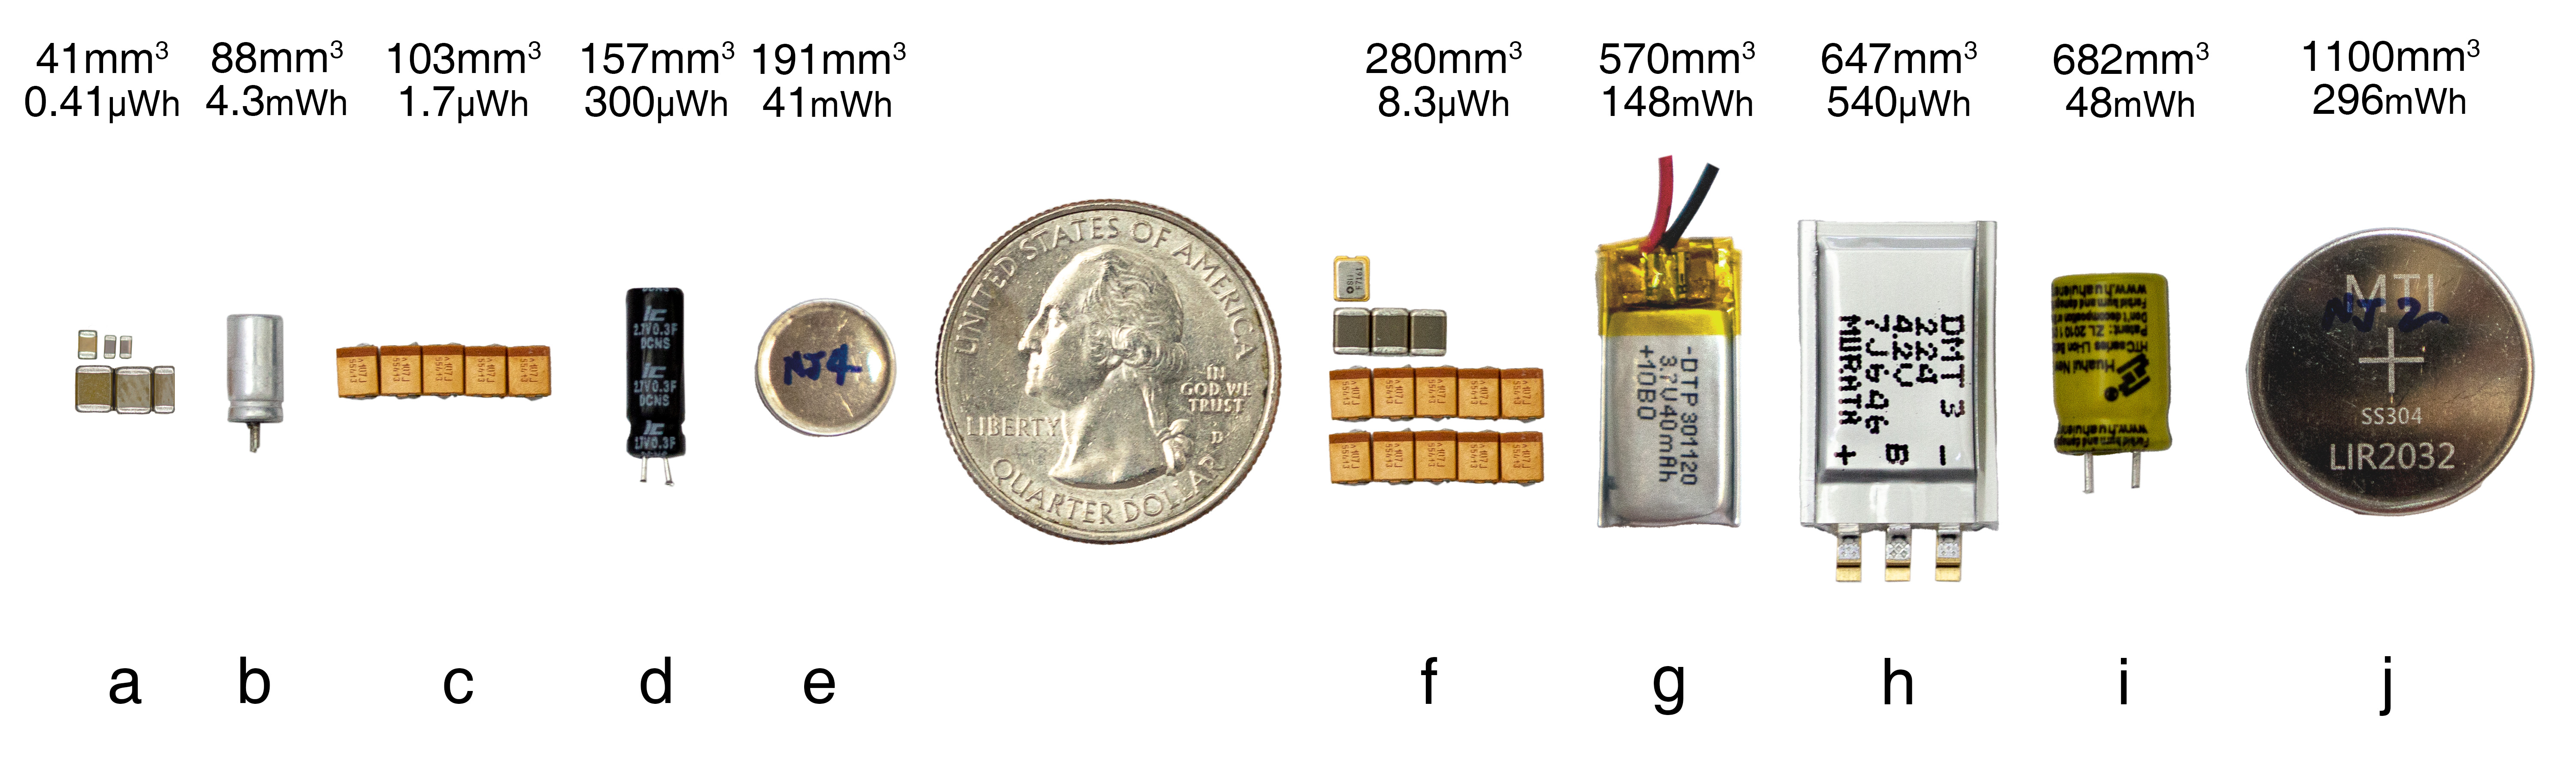
\includegraphics[width=\columnwidth]{figs/batteries/cap_lto_size_compare}
  \caption{
    A size comparison of energy storage methods including capacitors, supercapacitors, and batteries.
    \normalfont
    They are ordered left to right, by their
    (total) volume. Total volumes and energy storage are listed above the respective device.
    Configuration
    \textbf{(a)}, \textbf{(c)} and \textbf{(f)} represent the energy storage configurations used
    in the Flicker platfrom with BLE and several sensors~\cite{hesterFlicker17}, the Solar Monjolo~\cite{campbellEnergy14} and the Capybara temperature
    monitor and alarm~\cite{colinReconfigurable18}, which have total
    capacitances and energy capacities of 119\si{\micro\farad} (0.41\si{\micro\Wh} at 5~V), 500\si{\micro\farad} (1.7\si{\micro\Wh} at 5~V)
    and 8.8\si{\milli\farad} (8.3\si{\micro\Wh} at 2.6~V), respectively. Capacitors
    \textbf{(d)}~\cite{illinoisCap} and \textbf{(h)}~\cite{murataCap} are large
    supercapacitors available on the Capybara platform and have the
    capacitances and energy capacities of 300\si{\milli\farad} (300\si{\micro\Wh} at 2.7\si{\volt}) and 220\si{\milli\farad}
    (540\si{\micro\Wh} at 4.2\si{\volt}) respectively.  Devices \textbf{(b)} and \textbf{(i)} are 
    small LTO battery cells with 1.8\si{\milli\Ah} (4.3\si{\milli\Wh} at 2.4~V) and 20\si{\milli\Ah} (48\si{\milli\Wh}
    at 2.4\si{\volt}) capacity respectively~\cite{LTODatasheet2}. Devices \textbf{(e)} and \textbf{(j)} are small prototype Li-ion coin cells with 11\si{\milli\Ah} (41\si{\milli\Wh} at 3.7~V) and 80\si{\milli\Ah} (296\si{\milli\Wh} at 3.7~V) respectively~\cite{millibatNimbus}. Device \textbf{g} is a traditional Lithium Polymer pouch cell with 40\si{\milli\Ah} (148\si{\milli\Wh} at 3.7~V)~\cite{sparkfunPouch}.
    The LTO battery \textbf{(b)} and the Li-ion coin cell \textbf{(e)} are among the smallest of all configurations of energy storage
    presented here and also provide one to two orders of magnitude more energy capacity
    compared to \textbf{(f)}, the largest supercapacitor presented.
  }
\end{definefigure}

\begin{definefigure}{fig:battery:ragone}
\centering
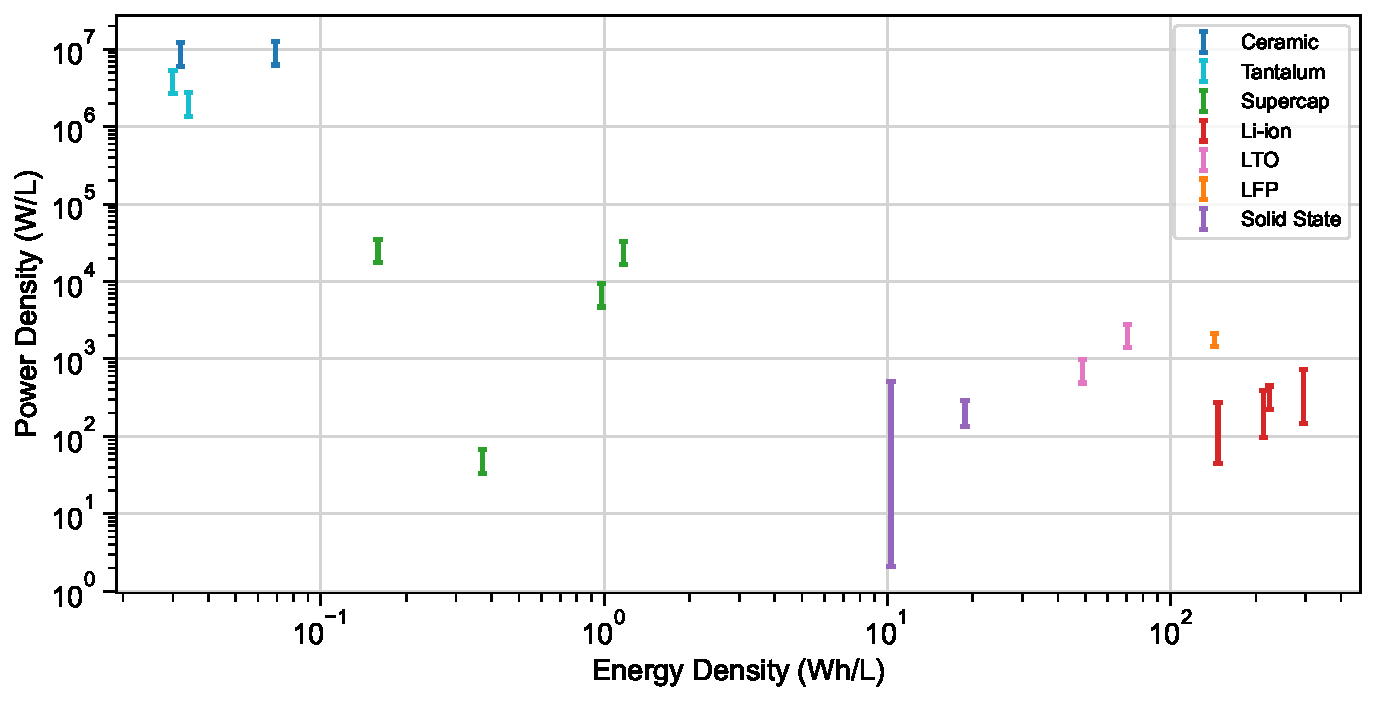
\includegraphics[width=\columnwidth]{figs/ragone}
\caption{}
\end{definefigure}